\exercisesection{1}


\begin{enumerate}
\def\labelenumi{\arabic{enumi}.}
\tightlist
\item
  In the commutative diagram (10) suppose that the ordered pair \((u', v')\) is an exact sequence and that \(v \circ u = 0\) . Show that
\end{enumerate}

\(\operatorname{Im}(b) \cap \operatorname{Im}(u') = b(\operatorname{Ker}(c \circ v))\) and \(\operatorname{Ker}(b) + \operatorname{Ker}(v) = b^{-1}(\operatorname{Im}(u' \circ a)).\)

\begin{enumerate}
\def\labelenumi{\arabic{enumi}.}
\setcounter{enumi}{1}
\tightlist
\item
  Consider a commutative diagram of commutative groups
\end{enumerate}

\pandocbounded{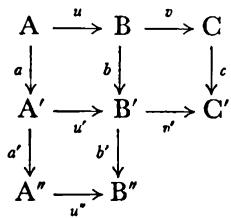
\includegraphics[keepaspectratio]{images/part001_696e1539.jpg}}

Suppose that: (1) \((u, v)\) and \((b, b')\) are exact sequences; (2) \(v' \circ u' = 0\) and \(a' \circ a = 0\) ; (3) \(c\) and \(u'\) are injective and \(a'\) is surjective. Show that under these conditions \(u''\) is injective.

\begin{enumerate}
\def\labelenumi{\arabic{enumi}.}
\setcounter{enumi}{2}
\tightlist
\item
  Consider a commutative diagram of commutative groups
\end{enumerate}

\pandocbounded{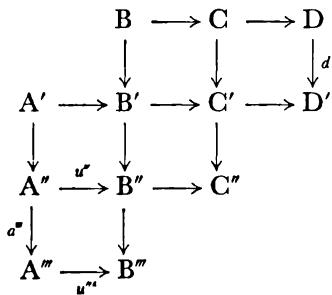
\includegraphics[keepaspectratio]{images/part001_1549be15.jpg}}

in which the rows and columns are assumed to be exact, d and \(u''\) injective and \(a''\) surjective. Show that under these conditions \(u'''\) is injective. Generalize this result.

\begin{enumerate}
\def\labelenumi{\arabic{enumi}.}
\setcounter{enumi}{3}
\tightlist
\item
  Consider a commutative diagram of commutative groups
\end{enumerate}

\pandocbounded{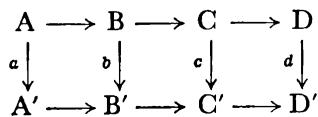
\includegraphics[keepaspectratio]{images/part001_0674edfc.jpg}}

where the two rows are assumed to be exact.

\begin{enumerate}
\def\labelenumi{(\alph{enumi})}
\item
  Show that, if \(a\) is surjective and \(b\) and \(d\) injective, then \(c\) is injective.
\item
  Show that, if \(d\) is injective and \(a\) and \(c\) surjective, then \(b\) is surjective.
\end{enumerate}

\begin{enumerate}
\def\labelenumi{\arabic{enumi}.}
\setcounter{enumi}{4}
\tightlist
\item
  Suppose that an exact sequence \(A^{\prime} \xrightarrow{u} A \xrightarrow{v} A^{\prime\prime} \to 0\) and two surjective homomorphisms \(B^{\prime} \xrightarrow{a^{\prime}} A^{\prime}, B^{\prime\prime} \xrightarrow{a^{\prime\prime}} A^{\prime\prime}\) are given, where A, A', A'', B', B'' are modules over the same ring. Show that, if \(B^{\prime\prime}\) is a projective module, there exists a surjective homomorphism \(a: B^{\prime} \oplus B^{\prime\prime} \to A\) such that the diagram
\end{enumerate}

\pandocbounded{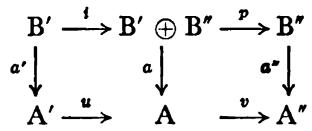
\includegraphics[keepaspectratio]{images/part001_093beead.jpg}}

is commutative (i and p being the canonical mappings).

\begin{enumerate}
\def\labelenumi{\arabic{enumi}.}
\setcounter{enumi}{5}
\tightlist
\item
  Suppose that an exact sequence \(0 \to A' \xrightarrow{u} A \xrightarrow{v} A''\) and two injective homomorphisms \(A' \xrightarrow{a'} C', A'' \xrightarrow{a''} C''\) are given, where \(A, A', A'', C', C''\) are modules over the same ring. Show that, if \(C'\) is an injective module (Algebra, Chapter II, § 2, Exercise 11), there exists an injective homomorphism \(a: A \to C' \oplus C''\) such that the diagram
\end{enumerate}

\pandocbounded{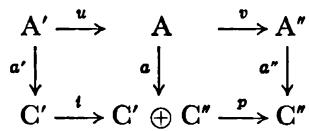
\includegraphics[keepaspectratio]{images/part001_5ee4bea9.jpg}}

are commutative (i and p being the canonical mappings).

\begin{enumerate}
\def\labelenumi{\arabic{enumi}.}
\setcounter{enumi}{6}
\tightlist
\item
  Let U, V, W be three commutative groups and \(f: \mathrm{U} \to \mathrm{V}\) , \(g: \mathrm{V} \to \mathrm{W}\) homomorphisms.
\end{enumerate}

\begin{enumerate}
\def\labelenumi{(\alph{enumi})}
\tightlist
\item
  Consider the diagram
\end{enumerate}

\pandocbounded{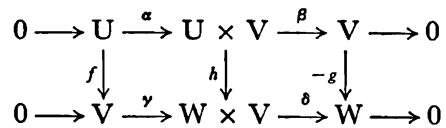
\includegraphics[keepaspectratio]{images/part001_5d67b0a0.jpg}}

where \(\alpha(u) = (u, f(u)), \beta(u, v) = v - f(u), \gamma(v) = (g(v), v), \delta(w, v) = w - g(v)\) , \(h(u, v) = (g(f(u)), v)\) . Show that this diagram is commutative and that its rows are exact.

\begin{enumerate}
\def\labelenumi{(\alph{enumi})}
\setcounter{enumi}{1}
\tightlist
\item
  Deduce from (a) and Proposition 2 of no. 4 an exact sequence
\end{enumerate}

\[
\begin{array}{c} 0 \to \operatorname{Ker} (f) \to \operatorname{Ker} (g \circ f) \to \operatorname{Ker} (g) \to \operatorname{Coker} (f) \to \operatorname{Coker} (g \circ f) \to \\ \operatorname{Coker} (g) \to 0. \end{array}
\]

Give a direct definition of this exact sequence.

